
\section{Experimental Tools}\label{method:tools}

In order to explore the large number of possible exchange instances described in
\S \ref{method:setup}, a sophisticated instance generation and solving framework
is needed. This section describes the design principles and implementation
details of a new software package called Cyclopts (\underline{Cycl}us
\underline{Opt}imization \underline{S}tudies). Cyclopts, written primarily in
Python with a C++ layer used to interface with Cyclus, provides a general
framework for sampling a parameter space, defining problem instances for a given
point in parameter space, and solving a problem instance under a variety of
conditions. While this section focuses on the Cyclopts workflow, implementation,
and high-throughput computing (HTC) capabilities, details specific to the
database layout and command line interface (CLI) are treated lightly. A full
treatment of the the database layout is provided in Appendix \ref{app:hdf5}, and
the CLI is detailed in Appendix \ref{method:tools:cli}.

\subsection{Terminology}\label{method:tools:term}

Cyclopts supports a two-tier definition of problem instances, borrowing terms
from biological classification. Problem \textit{families} describe a general
form of problem instance. For example, the Traveling Salesman Problem (TSP)
could be implemented as a problem family. In this analysis, the NFCTP is
considered the problem family, since any given instance of the NFCTP will have
the same general structure. Whether or not the LP or MILP formulation is used is
dependent on whether or not arcs in the Exchange Graph are labeled as exclusive
or not. If there are no exclusive arcs, the LP formulation is used; otherwise,
the MILP formulation is used.

Each problem family can have any number of \textit{species}. One can
conceptualize the relationship as a tree structure, in which families are parent
nodes and species are child nodes. A problem species defines the methodology for
generating \textit{instances} of a problem family. Using the TSP example above,
a problem species may be ``the greater Atlanta metropolitan area'', for which
the effect of regional gas prices may be studied. For the NFCTP study, front-end
and back-end exchanges form two separate species. Each species can have unique
parameters in addition to family-related parameters, as is the case for the two
species studied.

\subsection{Design}\label{method:tools:struc}

The full Cyclopts stack is comprised of three phases: generation of parameter
space, generation of instances, and execution of instances. The workflow begins
with user input detailing a range of values for a set of parameters. Cyclopts
then translates the input into a parameter space by enumerating all possible
combinations of parameters. For example, if parameters $x$ and $y$ have defined
values of $[1, 2]$ and $[3, 4, 5]$, respectively, Cyclopts will generate a
parameter space comprised of six points in $(x, y)$ notation: $(1, 3)$, $(1,
4)$, $(1, 5)$, $(2, 3)$, $(2, 4)$, and $(2, 5)$. Each point is then then
provided to a problem species in order to generate one or more problem
instances. Species are expected to define defaults for all parameters as user
input may define values for only a subset of available parameters.

Given a point in parameter space, an instance can be generated. If there are any
stochastic effects during instance generation, many instances may be
generated. Again, because parameters are species dependent, the logic of
instance generation from a set of parameters is the task of a problem
species. Following instance generation, instances can be executed. Cyclopts
supports multiple solution options by design. The same instance may be solved
with both a heuristic and a full optimization solver, for example. Once an
instance of a problem is defined, it is independent of any species-level
effects. Accordingly, instance execution and related logic is the domain of
problem families.

A summary of the high-level Cyclopts workflow and entities is presented in
Figure \ref{fig:lopts_desgin}. Note that objects generated as the workflow moves
from parameter space to instance solution form a tree structure.

\begin{figure}
  \begin{center}
    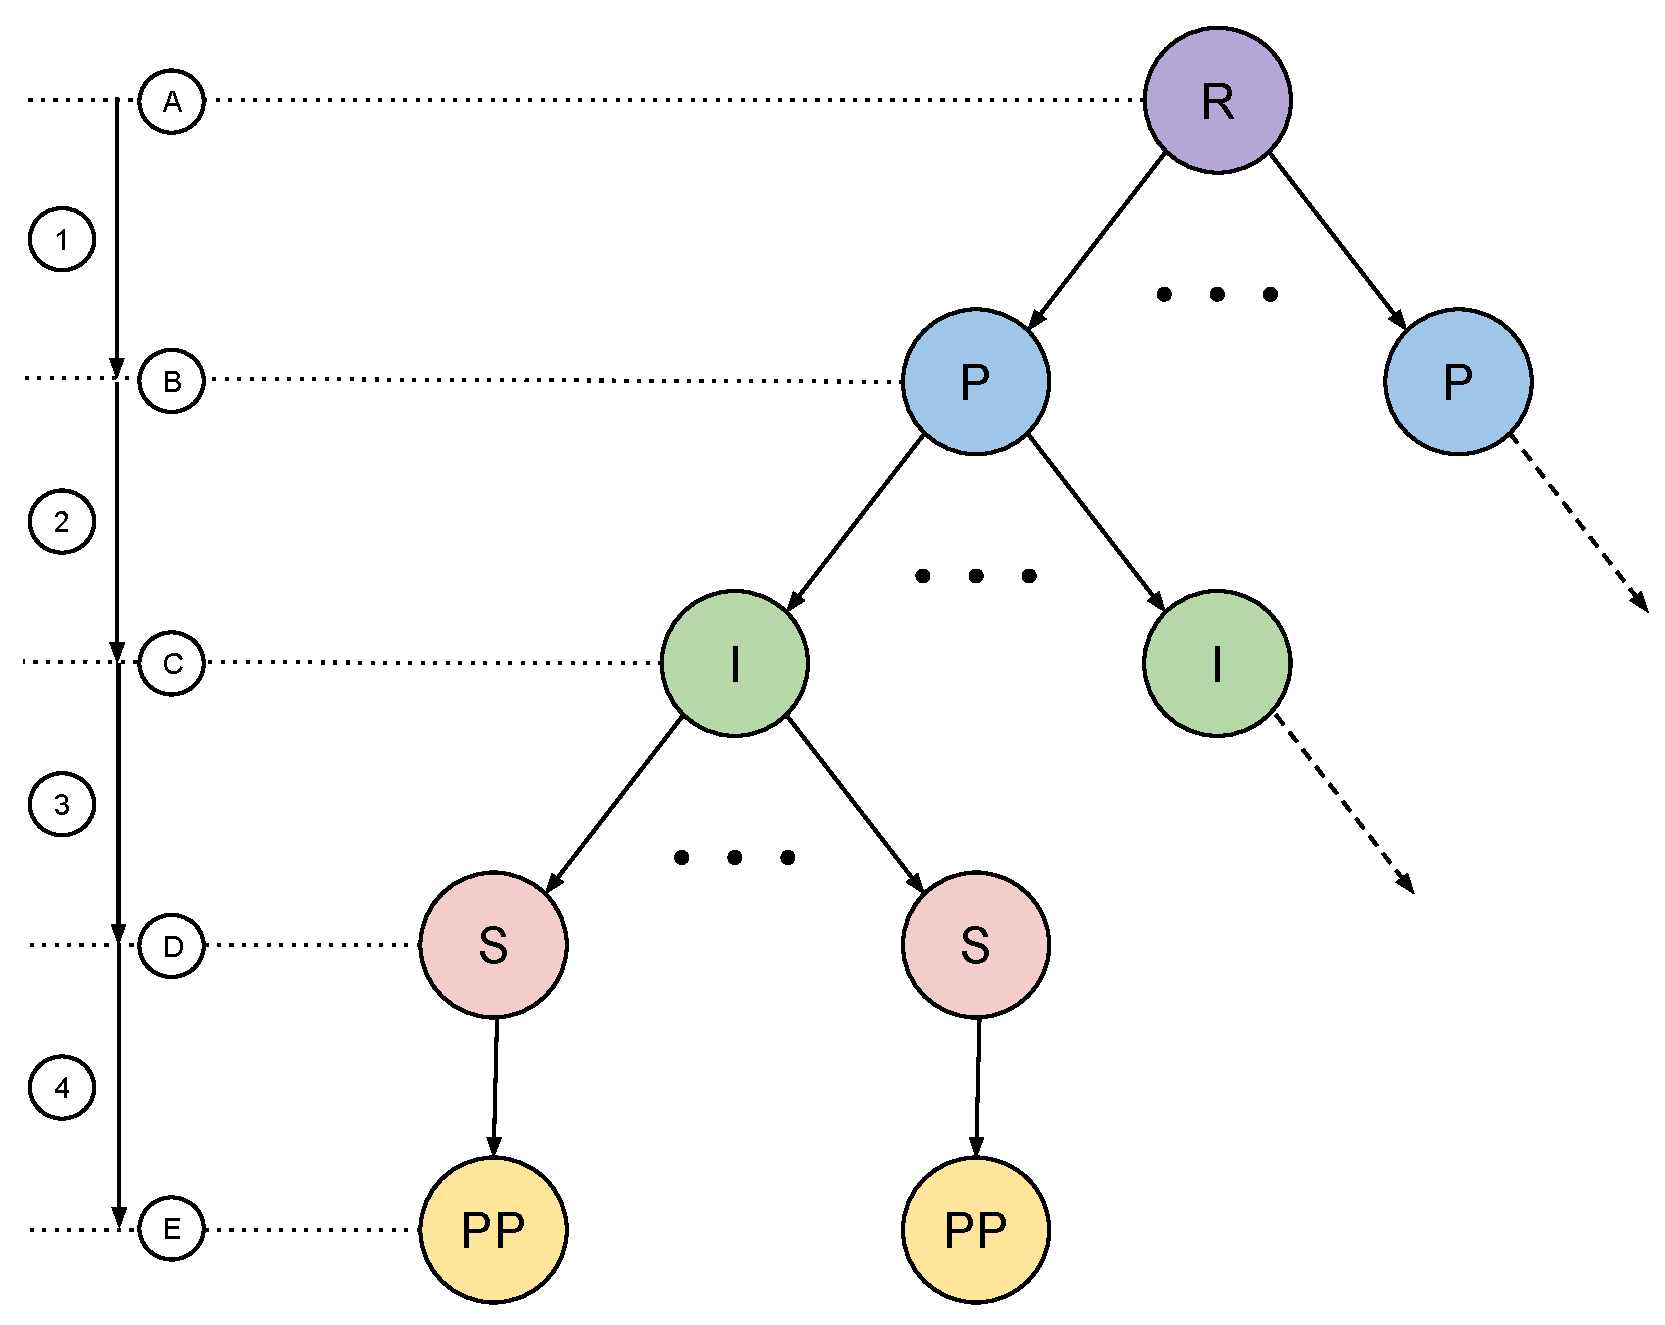
\includegraphics[width=\textwidth]{cyclopts_tree_flow.pdf}
    \caption{
      \label{fig:lopts_desgin}
      A graphical representation of the Cyclopts object tree-structure. For any
      parent node, there is a one-to-many mapping of children nodes. The node
      types in the tree structure are defined in Table
      \ref{tbl:lopts_nodes}. The actions associated with moving between each
      level are explained in Table \ref{tbl:lopts_actions}.}
  \end{center}
\end{figure}

\begin{table}[h!]
\centering
\caption{Cyclopts object tree structure node types as shown in Figure \ref{fig:lopts_desgin}.}
\label{tbl:lopts_nodes}
\begin{tabularx}{\columnwidth-10pt}{|c|c|X|} % line wraps second column if too long
\hline
\textbf{Label}    & \textbf{Node Type} & \textbf{Description}
\\ \hline
A & Root & A definition of the full parameter space as provided by a user.
\\ \hline
B & Parameter & A fully defined point in the parameter space.
\\ \hline
C & Instance & A fully defined instance of a given problem.
\\ \hline
D & Solution & A solution to an instance of a problem determined by an appropriate solver.
\\ \hline
E & Post-process & Post-processed information, given all parent nodes.
\\ \hline
\end{tabularx}
\end{table}

\begin{table}[h!]
\centering
\caption{Cyclopts actions generating child nodes as shown in Figure
  \ref{fig:lopts_desgin}. The Cyclopts entity, e.g., the family or species,
  associated with each action is also listed.}
\label{tbl:lopts_actions}
\begin{tabularx}{\columnwidth-10pt}{|c|X|c|} % line wraps second column if too long
\hline
\textbf{Label} & \textbf{Action} & \textbf{Entity Responsible}
\\ \hline
1 & Translate a parameter space into all possible points. & Cyclopts Core
\\ \hline
2 & Convert a parameter point into a number of problem instances. & Problem Species
\\ \hline
3 & Execute a problem instance given a solver and record the solution. & Problem Family
\\ \hline
4 & Post-process a solution and instance, recording relevant information. & Problem Family \& Species
\\ \hline
\end{tabularx}
\end{table}

\subsection{Persistence Mechanisms}\label{method:tools:hdf5}

While the root node in Figure \ref{fig:lopts_desgin} is generated from a
user-provided input file, each subsequent level in the hierarchy represents a
stateful object: a point in parameter space, a problem instance, and a
solution. Each stateful object can be written to and read from disc. Cyclopts
also incorporates a post-processing step, during which all related objects may
be analyzed and aggregate data may be collected and written to disc. While any
input/output (I/O) persistence mechanism is valid, Cyclopts is currently
implemented using the Hierarchical Data Format (HDF5) \cite{hdf5} via PyTables
\cite{pytables}.

Data in HDF5 is stored hierarchically, similar to a file system. At the root node
of the file-system-like structure, a \textit{group} is defined for problem family
and problem species data, named \code{Family} and \code{Species},
respectively. A \textit{dataset} for aggregate results named \code{Results} is
also defined. A path in HDF5 is designated in a UNIX-like manner. For example,
the path to \code{Family} would be \code{/Family}, indicating that the group is
directly under the root node, \code{/}. Further, groups are defined for each
kind of family and species. The DRE problem family records data in the group
\code{/Family/ResourceExchange}, front-end exchanges record data in the group
\code{/Species/StructuredRequest}, and back-end exchanges record data in the
group \code{/Species/StructuredSupply}. 

Each stateful object is given a Universally Unique Identifier (UUID) by which it
can be identified for future reading and analysis. The UUID is used in two
distinct capacities: as a \textit{primary key} in a dataset for future
identification or as the name of a group. Whether to aggregate data in one large
dataset or divide data into datasets for each object is a design decision
informed by practical performance. A study of the trade-offs between each
approach is presented in \S \ref{method:tools:hdf5:study}. As a result of that
study, for objects that are both read and written, the latter approach is taken.

A description of all data gathered for each family and species for conversion,
execution, and post-processing is detailed in Appendix \ref{app:hdf5}.

\subsubsection{Performance Studies}\label{method:tools:hdf5:study}

\textit{Chunk size} is a critical parameter of HDF5 datasets that affects I/O
performance. HDF5's storage layout is not contiguous; rather, data is separated
into equal-sized \textit{chunks}. Any reading or writing occurs on a chunk of
data, rather than accessing an entire dataset. Accordingly, choosing a reasonable
chunk size can greatly increase performance for known data access operations. In
PyTables, the \textit{compression level} of a dataset is also a tune-able
parameter that affects I/O performance. Compression, of course, reduces overall
database size. Therefore, an ideal compression is the largest possible that
retains acceptable performance.

Originally, all Cyclopts datasets used a UUID-as-primary-key layout. For
instance, rather than having tables with a layout described in Table
\ref{tbl:/Family/ResourceExchange/ExchangeArcs}, a single table with an extra
column naming the instance UUID was used. However, extremely long read times
were encountered when post processing data. The basic procedure for performing a
post-process operation included reading all rows associated with a UUID in an
exchange species dataset, reading all rows associated with the same UUID in an
exchange family dataset, selecting a value from each row (resulting in two
vectors), and performing a dot product operation.

In order to investigate possible chunk size and compression optimizations, a
small ($\sim$ MBs) dataset and a large ($\sim$ GBs) dataset were created. The
post-processing step was then run on 25 instances in each dataset. The operation
was timed using the UNIX \code{time} command. An initial chunksize for each
dataset was chosen to be proportional to the ratio of a normal L2 cache to row
size and a compression level of four was selected per suggestions from the
PyTables documentation \cite{tablesopt}. For the performance study, chunk size
and compression level were varied around these recommended values in order to
determine if any tuning was available. The results of the study on the small
dataset is shown in Figure \ref{fig:small_db}. The large dataset results is
shown in Figure \ref{fig:large_db}.

\begin{figure}
  \begin{center}
    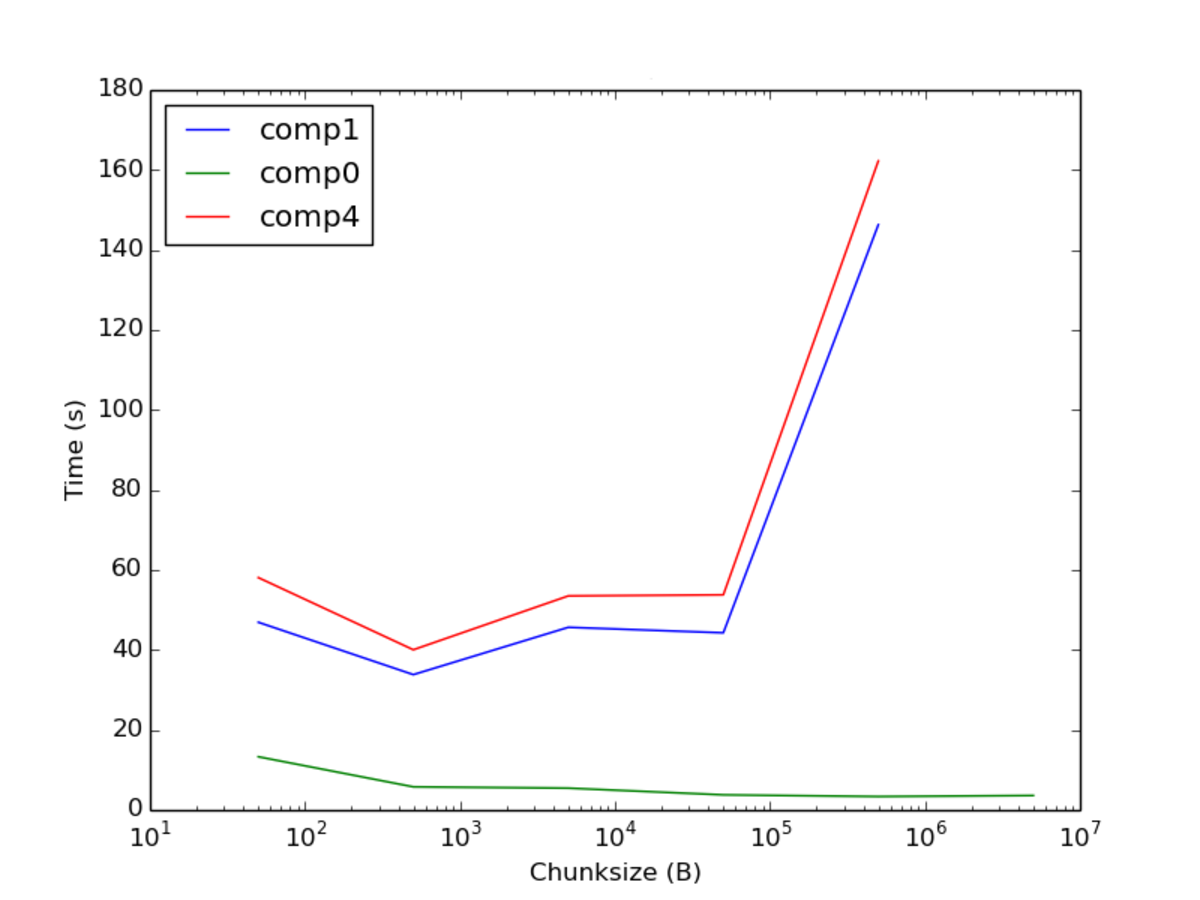
\includegraphics[width=0.85\textwidth]{small_all.pdf}
    \caption{
      \label{fig:small_db}
      Post-processing performance for 25 entries of a small-sized database for a 
      variety of compression levels and chunk sizes.}
  \end{center}
\end{figure}

\begin{figure}
  \begin{center}
    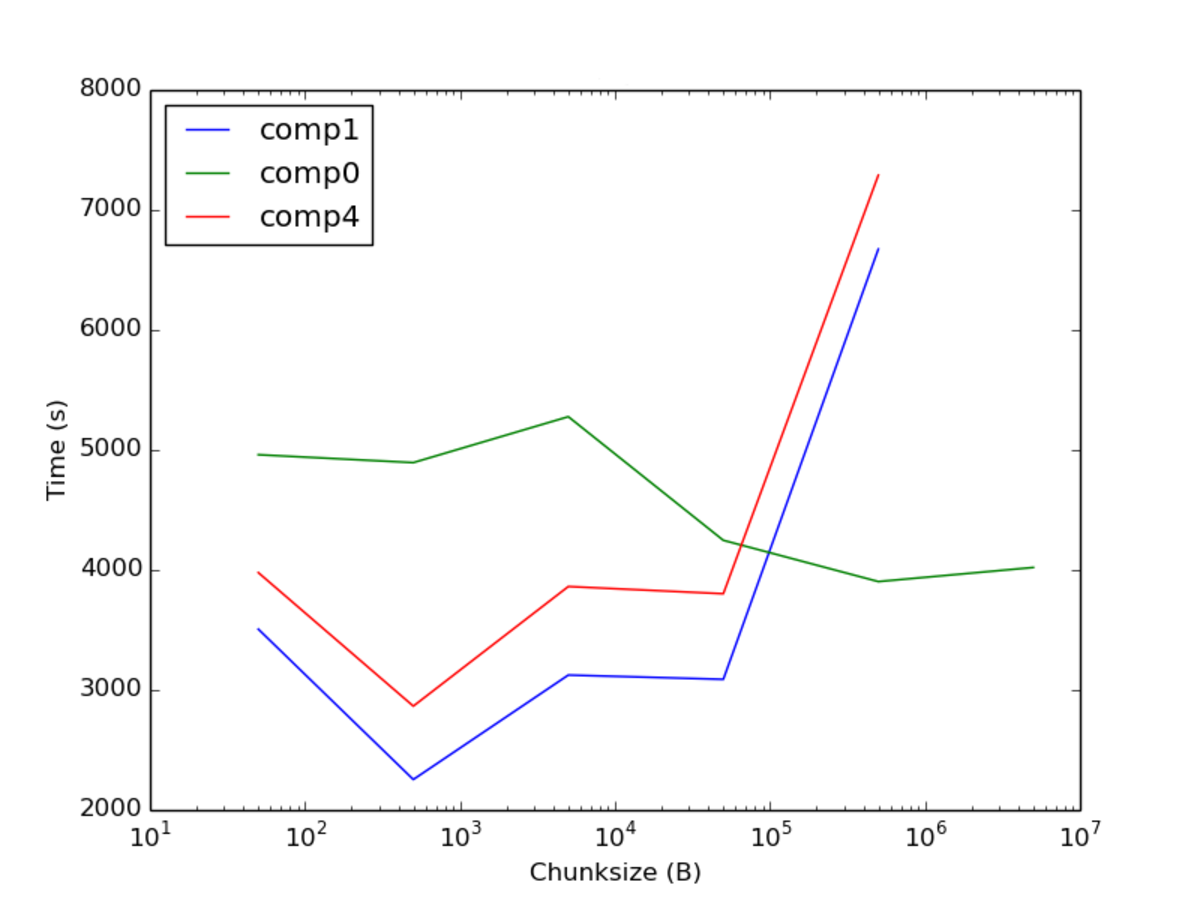
\includegraphics[width=0.85\textwidth]{large_all.pdf}
    \caption{
      \label{fig:large_db}
      Post-processing performance for 25 entries of a large-sized database for a
      variety of compression levels and chunk sizes.}
  \end{center}
\end{figure}

Assuming some level of compression, an ideal chunksize range is identified for
the small database of between $\sim 10^3 - 10^5$ bytes. Further the small
database example confirms that the study's methodology is well founded: an ideal
chunksize range is established. A similar optimal chunk size range is found for
the large database. However, note that in this exercise, only $\sim 0.25\%$ of
instances are post-processed. An optimal performance of $> 80$ seconds per
instance is unacceptable.

A number of strategies exist for trying to increase performance. A classic
strategy is pivoting the group-dataset structure such that data queries are made
upon an entire group rather than rows in a dataset. In this example, such a
pivot involves dividing the single, large dataset into $n$ datasets, where $n$
is the number of unique primary keys, i.e., UUIDs.

Accordingly, an additional performance test was conducted with a new database
layout. All datasets on which queries are made were pivoted such that new group
nodes were added for each UUID, and all data for that UUID was appended to a
dataset under the associated group. The post processing step was divided into
the read and vector-population operations associated with the exchange family
and the the read and vector-population operations associated with a species. The
exact same operations were applied to a large database with the column-based
layout and a large database with the group-based layout. Specific instances,
increasing in size, were identified to be post-processed. The group-based results
were compared with the column-based results and are shown in Figure
\ref{fig:col_grp}. The speed of each operation was compared directly for both
layout strategies. The ratio of the group-strategy running time to the column
strategy running time was then plotted. Therefore, a low ratio implies a large
time savings, and a ratio close to unity implies almost no time savings. Times
were calculated using the IPython magic \texttt{\%timeit} command.

\begin{figure}
  \begin{center}
    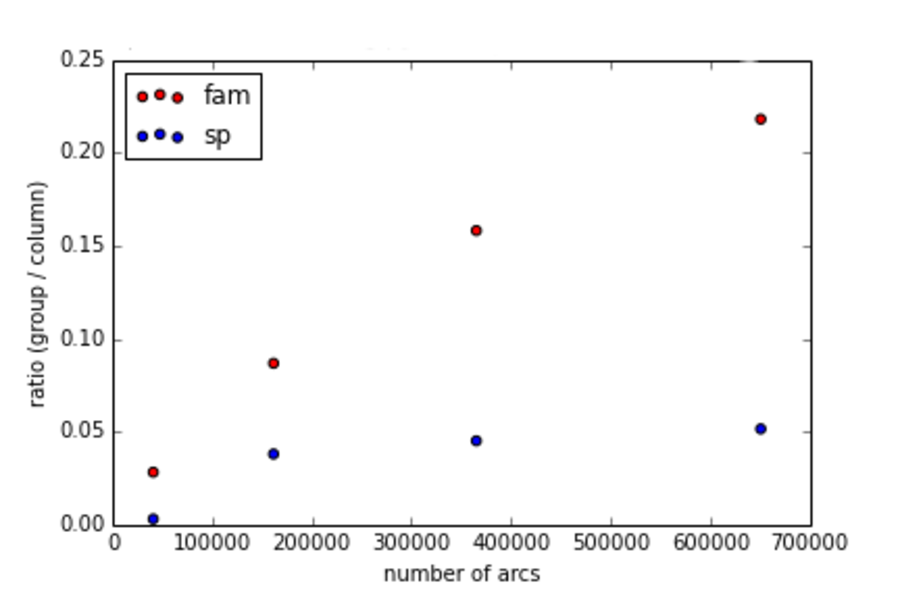
\includegraphics[width=0.85\textwidth]{grp_v_col_ratio.pdf}
    \caption{
      \label{fig:col_grp}
      The ratio of group-based queries to column-based queries as a function of
      problem size. A lower ratio indicates a faster process time for the group
      strategy over the column strategy.}
  \end{center}
\end{figure}

As can be seen, the group-based strategy performs quite well, over an order of
magnitude better than the column-based strategy for species
operations. Furthermore, species operations are shown to have a much larger
speedup relative to family operations. This artifact is due to the fact that at
the time of this analysis, solution values were stored \textit{only if} they
were nonzero. When read, a data structure must be allocated and populated for
each non-zero index rather than simply copying a block on data on disc. The
writing of family-based solution values has since been updated to also write
zero values to avoid this issue.

For the purposes of this study, the dataset-group pivot served the required
purpose. Post-processing now performs satisfactorily for the operations needed
and the database sizes experienced. However, if future performance issues arise,
other strategies may be investigated. Perhaps the most fruitful of these will be
returning to the single dataset layout and using PyTable's indexing feature. 

\subsection{Implementation}

Cyclopts defines abstract application programming interfaces (APIs) for both
families and species in the \code{ProblemFamily} and \code{ProblemSpecies}
classes, respectively. While many parts of an API are related to the workflow
discussed in \S \ref{method:tools:struc}, others are related to the persistence
mechanisms discussed in \S \ref{method:tools:hdf5}. The full API is described in
detail in the Cyclopts documentation \cite{cyclopts}. The \code{ExchangeFamily}
class implements a concrete, NFCTP-specific \code{ProblemFamily} interface. The
\code{StructuredRequest} class implements a concrete, front-end-exchange
interface of the \code{ProblemSpecies} class. Similarly, the
\code{StructuredSupply} implements a back-end interface to the class.

Given a point in parameter space, both the \code{StructuredSupply} and
\code{StructuredRequest} generate an instance of an \code{ExchangeGraph} per the
rules described in \S \ref{method:setup}. Cyclopts is nominally written in
Python and Cyclus is written in C++. In order to construct objects that can
interact with Cyclus, an interoperability layer is required. 

A series of C++ wrapper objects, namely arc, node, and group objects, are
defined which mirror the constituents of an \code{ExchangeGraph}, as described
in \S \ref{abm:dre:impl}. These objects are then translated into Cython
\cite{behnel2010cython} by use of the XDress software package
\cite{xdress}. Python can directly call into Cython libraries, similarly, Cython
can directly call C and C++ libraries. Hence, an interoperability layer is
established.

\subsubsection{Solvers and Performance Timing}

Once an instance of an \texttt{ExchangeGraph} has been generated, it can be
solved. Cyclopts supports three types of solvers: CoinCLP, CoinCBC, and the
\texttt{GreedySolver}, an implementation of the Greedy Heuristic in Cyclus. If
either the Greedy or CBC solvers are invoked, an appropriate instance of a
\texttt{ExchangeSolver} is constructed with the \textit{exclusive orders} flag
turned on. If the CLP solve is invoked, an associated \texttt{ExchangeSolver}
instance is constructed with the \textit{exclusive orders} flag turned off. In
short, CBC and Greedy solvers solve the MILP formulation of the NFCTP, and the
CLP solver solves the LP formulation.

Given an instance of an \texttt{ExchangeGraph} and \texttt{ExchangeSolver}, the
\texttt{Solve} method of the \texttt{ExchangeSolver} is invoked. Before and
after the \texttt{Solve} function call, the \texttt{CoinCpuTime()} function is
called and the result is stored. The difference between the two resulting values
is recorded as the time required to determine a solution. The implementation of
the \texttt{CoinCpuTime()} function is open and easily available
\cite{coinosi}. It simply adds the seconds and microseconds fields of the
\texttt{ru\_utime} structure populated by the standard UNIX
\texttt{getrusage()} function.

\subsection{High Throughput Computing}\label{method:tools:htc}

Cyclopts can be executed locally using the \code{cyclopts exec} command-line
interface (CLI) described in Appendix \ref{method:tools:cli}. When exploring a
large parameter space, of which each point can generate a large number of unique
instances, local execution on a single machine is insufficient. In order to
overcome this limitation, support for HTCondor-based systems has been implemented
in Cyclopts and available using the \code{cyclopts condor-submit} CLI. HTCondor
\cite{condor-practice} is a high throughput computing (HTC) framework that
supports sophisticated job scheduling over a very large, distributed network of
individual and clustered computers.

HTC systems are ideal for analyses in which many independent executions must be
performed. Upon completion, the results may be aggregated and analyzed. The
resource-exchange use case fits such a design specification with a single
caveat: because it is a first-of-a-kind performance analysis, timing results are
crucial. Therefore, the systems on which instances are executed must be
equivalent in order to compare different timing results. Support is provided in
Cyclopts for identifying execute nodes that conform to a series of architecture
and related constraints in order to support this analysis limitation.

\subsubsection{Remote Execution and Operation}

In order to efficiently schedule a large number of optimization problems, the
WorkQueue framework \cite{bui_work_2011} is utilized. WorkQueue is a
HTCondor-aware master-worker implementation. A master process exists at some
location and manages the scheduling jobs to be run. Workers, in the form of
persistent HTCondor jobs, ask the master for the next job to be run after a
previous job has been completed. A master-worker system is especially useful in
HTCondor environments in which resources are limited and must be specifically
targeted, as is the case with the aforementioned timing studies.

Cyclopts launches a master process that requires a series of execute nodes to
target, a problem instance database, and a list of solvers to execute on each
instance. A copy of the instance database is sent to every targeted execute
node. Note that an execute node may have many execution threads, each of which
can be used to execute instances individually. The master manages an instance
queue from which jobs are provided to workers. Upon completion, a worker will
request a new instance of the master. The full set of instances in a database
are hence efficiently executed.

\subsubsection{Packaging and Environment}

A common issue in remote execution environments is package dependency. When
access to an execution node is provided, a user must assume that only the barest
of environments exist. For example, if a user is provided an Ubuntu-based
execution node, the user generally must assume that it is a fresh Ubuntu
installation. Accordingly, package management in a highly distributed,
heterogeneous environment is a difficult problem.

Luckily, solutions exist for distributed package management. Cyclopts utilizes
the Code, Data, and Environment (CDE) \cite{cde} tool to manage its execution
environment. CDE provides a virtualized environment based on the local execution
of a command. Using CDE with the given command, all libraries and utilities used
during the process execution are monitored. Upon process exit, every object in
the filesystem that was invoked is copied into a virtual environment. That
virtual environment can then be packaged and distributed. Upon landing on a
foreign system, a user can enter the CDE environment and execute the supported
command.

Cyclopts provides a CLI, \code{cyclopts cde}, that will package Cyclopts itself
into a virtual environment and ship the environment to a HTCondor submit node. As
part of the Cyclopts HTCondor job execution, the CDE environment is copied to each
execute node. It is therefore easy to incorporate changes in a local copy of
Cyclopts to the corresponding remote execution.
